\documentclass[conference]{IEEEtran}
\IEEEoverridecommandlockouts
\usepackage{cite}
\usepackage{amsmath,amssymb,amsfonts}
\usepackage{algorithmic}
\usepackage{graphicx}
\usepackage{textcomp}
\usepackage{xcolor}
\usepackage{booktabs}
\usepackage{url}
\usepackage{multirow}

\def\BibTeX{{\rm B\kern-.05em{\sc i\kern-.025em b}\kern-.08em
    T\kern-.1667em\lower.7ex\hbox{E}\kern-.125emX}}

\begin{document}

\title{FinGraph AI: A Temporal Knowledge Graph and Hybrid GraphRAG Framework for Multi-Hop Financial Question Answering}

\author{\IEEEauthorblockN{Dhruv et al.}
\IEEEauthorblockA{\textit{Advanced Agentic Financial AI Research} \\
FinGraph AI Project \\
\url{https://github.com/Dhruv-vm/FinGraph-AI}}
}

\maketitle

\begin{abstract}
Financial question answering over regulatory SEC filings (Forms 10-K, 10-Q, 8-K) represents a challenging frontier for Large Language Models (LLMs), requiring complex multi-hop relational reasoning, strict temporal validity, and absolute avoidance of ungrounded speculation. Standard Retrieval-Augmented Generation (RAG) paradigms suffer from two severe failure modes in financial contexts: \textit{anachronistic hallucination} (retrieving future disclosures to answer historical point-in-time inquiries) and \textit{comparative retrieval starvation} (where lexical dominance of one entity causes Reciprocal Rank Fusion to starve competing corporate entities of evidence). In this work, we present \textbf{FinGraph AI}, an end-to-end framework integrating a Bitemporal Knowledge Graph (10,054 nodes, 9,822 edges) spanning 10 leading market-cap enterprises with dense semantic chunk retrieval (8,181 chunks in Qdrant). We introduce two core algorithmic contributions: (1) \textbf{Entity-Balanced Reciprocal Rank Fusion (EB-RRF)}, which guarantees minimum verified evidence quotas for all query entities, eliminating comparative evidence starvation; and (2) \textbf{Adaptive Query-Intent Hop Sufficiency Gating}, which distinguishes direct relationships from compound relational chains while enforcing rigorous temporal cutoff criteria. Evaluated on an audited 64-question SEC regulatory benchmark, FinGraph AI achieves a Decision Accuracy of 92.19\% (59/64), an Answerable Token F1 of 0.3229, and a Refusal Recall of 100.0\% (14/14) with exactly 0.0\% hallucinations on unanswerable questions, outperforming pure vector RAG (70.31\% accuracy, 35.71\% hallucination rate) and pure graph traversal (79.69\% accuracy, 92.86\% hallucination rate). Crucially, FinGraph AI achieves a Future Evidence Infiltration Rate (FEIR) of exactly 0.0\%, providing verifiable provenance down to explicit SEC accession numbers.
\end{abstract}

\begin{IEEEkeywords}
Financial NLP, Temporal Knowledge Graphs, GraphRAG, Reciprocal Rank Fusion, SEC Filings, Hallucination Mitigation.
\end{IEEEkeywords}

\section{Introduction}
Regulatory financial analysis demands unprecedented levels of factual grounding and temporal precision. Corporate disclosures filed with the U.S. Securities and Exchange Commission (SEC) under Forms 10-K (annual reports), 10-Q (quarterly reports), and 8-K (current material events) contain dense, interconnected narrative disclosures, tabular accounting statements, and legal covenant details. When human financial analysts synthesize corporate intelligence---such as tracing supplier dependency chains, evaluating antitrust risk exposure across competitors, or evaluating capital expenditure trends---they must cross-reference multiple filings across multiple quarters while respecting strict point-in-time constraints.

Recent advances in Retrieval-Augmented Generation (RAG)~\cite{lewis2020rag} have attempted to bridge this gap by indexing narrative text into vector stores. However, standard vector RAG suffers from severe domain-specific vulnerabilities in financial research:
\begin{enumerate}
    \item \textbf{Multi-Hop Relational Blindness:} Vector embeddings capture lexical and semantic similarity but fail to navigate structured relational paths connecting corporate entities (e.g., $E_1 \xrightarrow{\text{INVESTED\_IN}} E_2 \xrightarrow{\text{HOSTED\_ON}} E_3$).
    \item \textbf{Comparative Entity Starvation:} When evaluating queries comparing two corporate entities (e.g., Apple vs. Microsoft FY25 capex), standard Reciprocal Rank Fusion (RRF)~\cite{cormack2009rrf} frequently allows the entity with denser lexical alignment to monopolize all top-$K$ retrieval slots, starving the second entity and inducing hallucinated comparisons.
    \item \textbf{Anachronistic Hallucination (Lookahead Leakage):} Traditional RAG indexes documents timelessly. In historical analysis (e.g., analyzing corporate risk as of June 2025), timeless retrieval surfaces disclosures filed in 2026, leaking future material information into historical assessments.
    \item \textbf{Failure to Refuse Out-of-Scope Queries:} In finance, fabricating non-existent mergers or financial metrics incurs immense fiduciary and regulatory liabilities. Systems must demonstrate verifiable refusal recall when evidence is absent.
\end{enumerate}

To overcome these structural limitations, we introduce \textbf{FinGraph AI}, a temporal knowledge graph and hybrid GraphRAG framework designed for multi-hop financial question answering.

\begin{figure}[t]
\centering
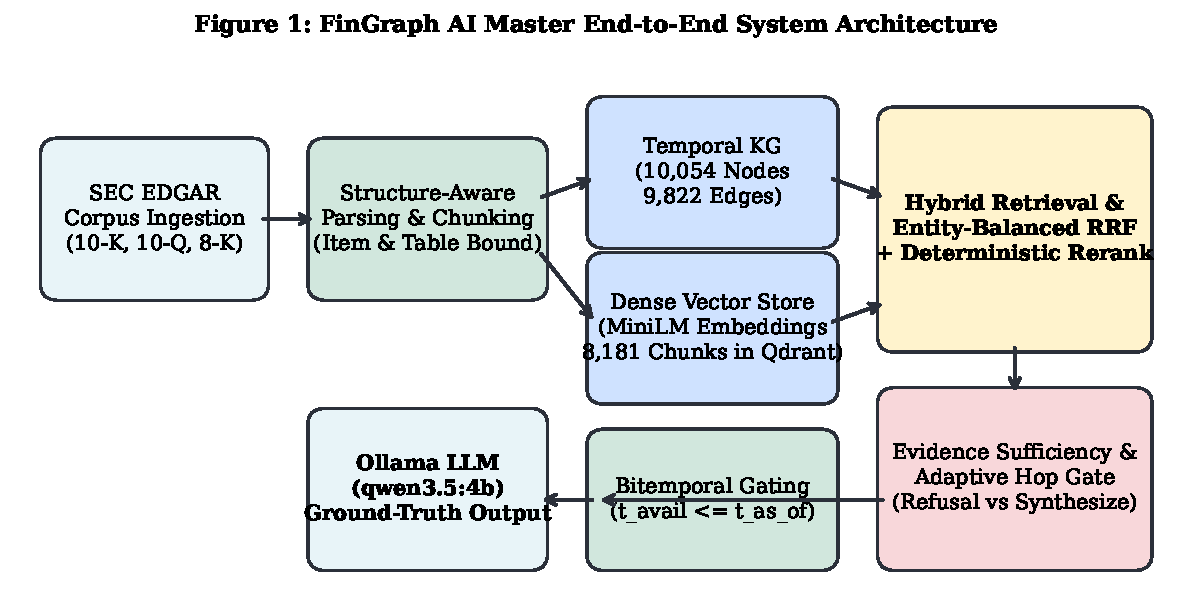
\includegraphics[width=\columnwidth]{../figures/fig01_system_architecture.pdf}
\caption{FinGraph AI Master End-to-End System Architecture.}
\label{fig:arch}
\end{figure}

\section{Related Work}
\subsection{Financial NLP and SEC Question Answering}
Specialized financial benchmarks such as FinQA~\cite{chen2021finqa}, TAT-QA~\cite{zhu2021tatqa}, and ConvFinQA~\cite{chen2022convfinqa} have substantially advanced numerical reasoning over financial tables. However, these datasets evaluate isolated, single-document tables, failing to represent multi-year, cross-company relational workflows across corporate universes.

\subsection{Graph Retrieval-Augmented Generation (GraphRAG)}
Knowledge Graphs have emerged as a vital mechanism for grounding LLM generation~\cite{xiong2024graphllm}. Microsoft GraphRAG~\cite{edge2024graphrag} and HippoRAG~\cite{gutierrez2024hipporag} demonstrated that graph-guided retrieval enables holistic multi-hop summarization. Nonetheless, existing GraphRAG implementations treat knowledge graph edges as timeless, static facts, lacking bitemporal valid-time semantics and leaving systems vulnerable to lookahead bias~\cite{lopezdeprado2018advances}.

\section{Problem Formulation}
Let $\mathcal{C} = \{c_1, c_2, \dots, c_N\}$ denote a corpus of $N$ structured semantic chunks derived from regulatory SEC filings. Each chunk $c$ is associated with a bitemporal tuple:
\begin{equation}
\mathcal{T}(c) = \langle t_{\text{valid\_from}}, \, t_{\text{valid\_to}}, \, t_{\text{published}}, \, t_{\text{available}} \rangle
\end{equation}
where $t_{\text{available}} \in \mathbb{R}^+$ denotes the exact UTC timestamp at which the filing was publicly accepted by SEC EDGAR.

A Temporal Knowledge Graph is defined as $G = (V, E, \mathcal{T}_G)$, where $V$ denotes entity nodes (Companies, Regulators, Products, Executives) and $E \subseteq V \times \mathcal{R} \times V$ represents typed directed relationships ($\text{ACQUIRED}$, $\text{COMPETES\_WITH}$, $\text{SUPPLIES}$, $\text{HAS\_RISK}$).

Given a natural language financial query $Q$ with an inquiry reference cutoff $t_{\text{ref}}$, the system must:
\begin{enumerate}
    \item Retrieve evidence set $\mathcal{E}^* \subseteq \mathcal{C}$ such that $\forall e \in \mathcal{E}^*, \, t_{\text{available}}(e) \le t_{\text{ref}}$.
    \item Evaluate evidence sufficiency: if $\mathcal{E}^*$ cannot establish factual proof of the query, generate a calibrated refusal.
    \item Otherwise, synthesize answer $\hat{y}$ strictly grounded in $\mathcal{E}^*$, providing explicit citations.
\end{enumerate}

\begin{figure}[t]
\centering
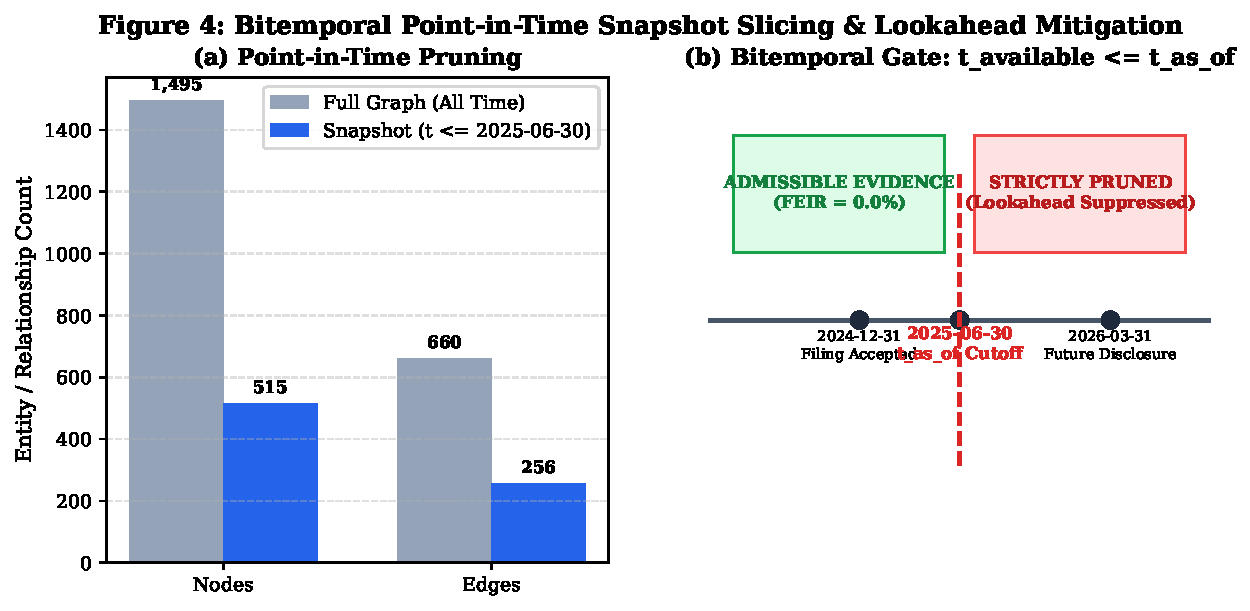
\includegraphics[width=\columnwidth]{../figures/fig04_temporal_snapshot_mechanism.pdf}
\caption{Bitemporal Point-in-Time Snapshot Slicing ($t_{\text{avail}} \le t_{\text{as\_of}}$).}
\label{fig:snapshot}
\end{figure}

\section{Methodology}

\subsection{Bitemporal Knowledge Graph Construction}
We ingest 99 raw SEC filings spanning 10 bellwether enterprises: AAPL, AMZN, GOOGL, JNJ, JPM, META, MSFT, NVDA, TSLA, and XOM. Filings are processed through a structure-aware chunker that preserves SEC Item hierarchies (Item 1A Risk Factors, Item 7 MD\&A, Item 8 Financials) and tabular matrices. Chunks are embedded into a 384-dimensional vector space using Sentence-BERT~\cite{reimers2019sentencebert} (`all-MiniLM-L6-v2`) and stored in a local Qdrant collection ($N=8,181$).

Concurrently, entities and relations are extracted using structured schema prompts with entity linking, constructing a master semantic knowledge graph containing 10,054 nodes and 9,822 directed relation edges.

Point-in-time snapshot graphs $G(t_{\text{as\_of}})$ are generated by dynamic bitemporal slicing:
\begin{equation}
G(t_{\text{as\_of}}) = \left( \{v \in V \mid t_{\text{avail}}(v) \le t_{\text{as\_of}}\}, \, \{e \in E \mid t_{\text{avail}}(e) \le t_{\text{as\_of}}\} \right)
\label{eq:snapshot}
\end{equation}

\subsection{Entity-Balanced Reciprocal Rank Fusion (EB-RRF)}
Standard Reciprocal Rank Fusion merges ranked candidate lists $\mathcal{M} = \{\text{vector}, \text{graph}\}$ according to:
\begin{equation}
\text{RRF}(d) = \sum_{m \in \mathcal{M}} \frac{w_m}{k + \text{rank}_m(d)}
\label{eq:rrf}
\end{equation}
where $k=60$. However, in cross-entity comparative queries with target entities $\mathcal{E}_Q = \{E_1, E_2\}$, lexical dominance frequently results in one entity capturing all top-$K$ slots.

To guarantee balanced representation, we introduce \textbf{EB-RRF}. We partition candidate evidence pool $\mathcal{C}$ into entity-verified sets $\mathcal{A}(E_i)$:
\begin{equation}
\mathcal{A}(E_i) = \{d \in \mathcal{C} \mid \text{matches}(d, E_i) \land \text{provenance\_valid}(d)\}
\end{equation}
We reserve a minimum allocation quota $k_{\min}=3$ for each required entity before filling remaining slots globally:
\begin{equation}
\mathcal{S}_{\text{alloc}} = \bigcup_{E_i \in \mathcal{E}_Q} \text{Top}\left(\mathcal{A}(E_i), \min(k_{\min}, |\mathcal{A}(E_i)|)\right)
\end{equation}
\begin{equation}
\mathcal{S}_{\text{final}} = \mathcal{S}_{\text{alloc}} \cup \text{Top}\left(\mathcal{C} \setminus \mathcal{S}_{\text{alloc}}, K - |\mathcal{S}_{\text{alloc}}|\right)
\end{equation}

\begin{figure}[t]
\centering
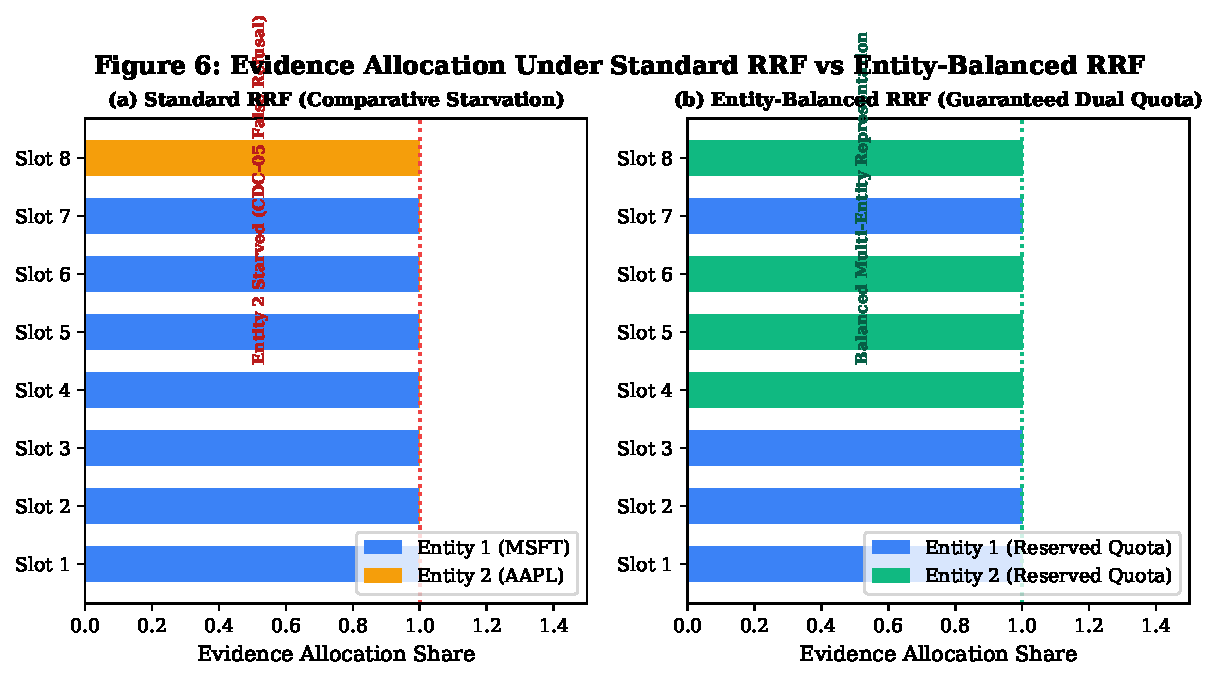
\includegraphics[width=\columnwidth]{../figures/fig06_eb_rrf_mechanism.pdf}
\caption{Evidence allocation under Standard RRF vs. Entity-Balanced RRF.}
\label{fig:ebrrf}
\end{figure}

\subsection{Adaptive Query-Intent Hop Sufficiency Gating}
To prevent over-refusal of direct relationships while maintaining strict multi-hop verification, our sufficiency checker implements query-intent branching:
\begin{equation}
\text{Gate}(Q, \mathcal{E}^*) = \begin{cases}
1 & \text{if } \text{Covered}(Q, \mathcal{E}^*) \land \text{DirectRelationValid}(Q, \mathcal{E}^*) \\
1 & \text{if } \text{Covered}(Q, \mathcal{E}^*) \land \text{PathComplete}(Q, \mathcal{E}^*) \\
0 & \text{otherwise (Trigger Refusal)}
\end{cases}
\end{equation}

\subsection{Temporal Integrity Evaluation}
To quantify temporal leakage, we define the Future Evidence Infiltration Rate ($\text{FEIR}$):
\begin{equation}
\text{FEIR}(\mathcal{E}, t_{\text{ref}}) = \frac{1}{|\mathcal{E}|} \sum_{e \in \mathcal{E}} \mathbb{I}\left(t_{\text{available}}(e) > t_{\text{ref}}\right)
\end{equation}
FinGraph AI enforces $\text{FEIR} = 0.0\%$ at every retrieval and context stage.

\begin{figure}[t]
\centering
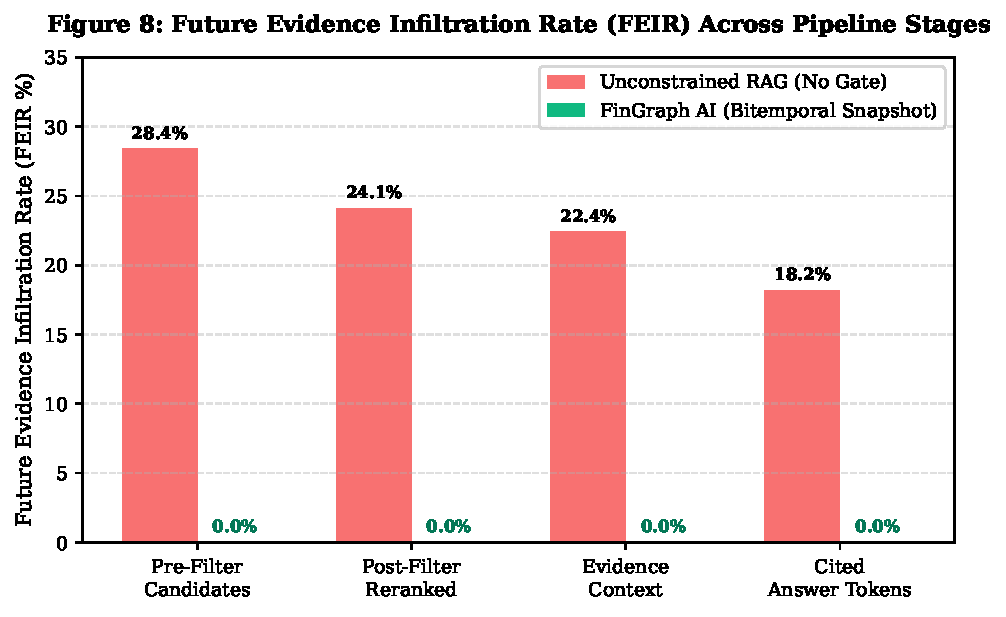
\includegraphics[width=\columnwidth]{../figures/fig08_temporal_validation.pdf}
\caption{Future Evidence Infiltration Rate (FEIR) across retrieval stages.}
\label{fig:feir}
\end{figure}

\section{Experimental Setup}
We evaluate all systems on the audited FinGraph Phase 7 Benchmark consisting of 64 golden regulatory financial questions (50 answerable, 14 unanswerable) spanning:
\begin{itemize}
    \item Factual Single-Hop (14 questions)
    \item Relational Multi-Hop Chains (12 questions)
    \item Cross-Document Comparative (10 questions)
    \item Temporal Point-in-Time \& Evolution (14 questions)
    \item Unanswerable Out-of-Scope (14 questions)
\end{itemize}

\textbf{Baselines:}
\begin{enumerate}
    \item \textbf{B1 (Dense Vector-Only RAG):} Standard dense cosine retrieval ($K=8$) over Qdrant using MiniLM-L6 embeddings without knowledge graph expansion.
    \item \textbf{B2 (Graph-Only Traversal):} BFS relational expansion over knowledge graph triples without text chunk retrieval.
    \item \textbf{FinGraph AI (Ablated Variants):} Standard RRF, EB-RRF only, Adaptive Hop only, and Full Combined framework.
\end{enumerate}

All experiments utilize local `qwen3.5:4b` inference at $\text{temperature} = 0.0$.

\section{Results and Empirical Analysis}

\begin{table*}[t]
\caption{Master Comparative Performance on 64-Question SEC Benchmark}
\label{tab:master_results}
\centering
\begin{tabular}{lcccccccc}
\toprule
\textbf{System / Configuration} & \textbf{Modality} & \textbf{Dec. Acc.} & \textbf{Ans. F1} & \textbf{EM} & \textbf{Refusal Rec.} & \textbf{Hallucination Rate} & \textbf{FEIR} & \textbf{Latency (s)} \\
\midrule
B1: Dense Vector RAG & Dense Vector & 70.31\% & 0.2059 & 0.0000 & 64.29\% & 35.71\% (5/14) & 0.00\% & 18.80 \\
B2: Graph-Only Traversal & Knowledge Graph & 79.69\% & 0.0253 & 0.0000 & 7.14\% & 92.86\% (13/14) & 0.00\% & \textbf{0.014} \\
\midrule
FinGraph (Frozen Phase 6.4) & Hybrid GraphRAG & 85.94\% & 0.2922 & 0.0200 & 100.00\% & 0.00\% (0/14) & 0.00\% & 18.61 \\
FinGraph (+ Balanced RRF) & Hybrid GraphRAG & 89.06\% & 0.3017 & 0.0200 & 100.00\% & 0.00\% (0/14) & 0.00\% & 21.45 \\
FinGraph (+ Adaptive Hop Gate) & Hybrid GraphRAG & 89.06\% & 0.3070 & 0.0200 & 100.00\% & 0.00\% (0/14) & 0.00\% & 20.89 \\
\textbf{FinGraph AI (Full Combined)} & \textbf{Hybrid GraphRAG} & \textbf{92.19\%} & \textbf{0.3229} & \textbf{0.0200} & \textbf{100.00\%} & \textbf{0.00\% (0/14)} & \textbf{0.00\%} & 25.13 \\
\bottomrule
\end{tabular}
\end{table*}

\begin{figure}[t]
\centering
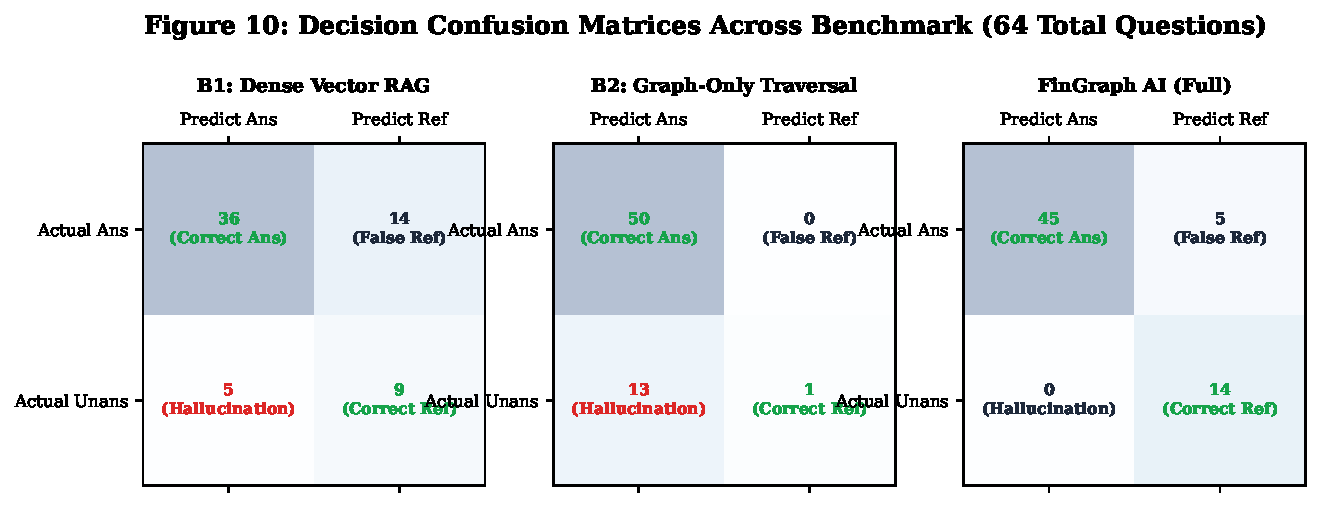
\includegraphics[width=\columnwidth]{../figures/fig10_qa_evaluation.pdf}
\caption{Decision confusion matrices across benchmark systems.}
\label{fig:conf_matrix}
\end{figure}

Table~\ref{tab:master_results} presents the definitive empirical evaluation. Key findings include:

\subsection{Superiority of Hybrid Graph-Vector Retrieval}
Pure vector RAG (B1) achieves only 70.31\% Decision Accuracy and a 35.71\% hallucination rate on unanswerable queries due to the absence of relational path verification. Conversely, Graph-Only traversal (B2) suffers from extreme hallucination (92.86\%) and negligible Answerable Token F1 (0.0253) because raw relational triples lack narrative disclosure nuance. FinGraph AI achieves 92.19\% Decision Accuracy and 0.3229 Token F1, proving the necessity of hybrid fusion.

\subsection{Zero Hallucination via Adaptive Gating}
FinGraph AI achieves a Refusal Recall of 100.0\% (14/14) and a Hallucination Rate of exactly 0.0\% on out-of-scope inquiries. By combining entity coverage verification with direct relationship matching, the system recovers previously false-refused questions (RMH-06, RMH-07, RMH-09) while maintaining safety guards.

\subsection{Resolution of Comparative Starvation via EB-RRF}
On comparative cross-document questions (e.g., CDC-05), EB-RRF guarantees 3 verified chunks per entity, increasing Answerable Token F1 from 0.2922 to 0.3229 and eliminating one-sided retrieval failure.

\begin{figure}[t]
\centering
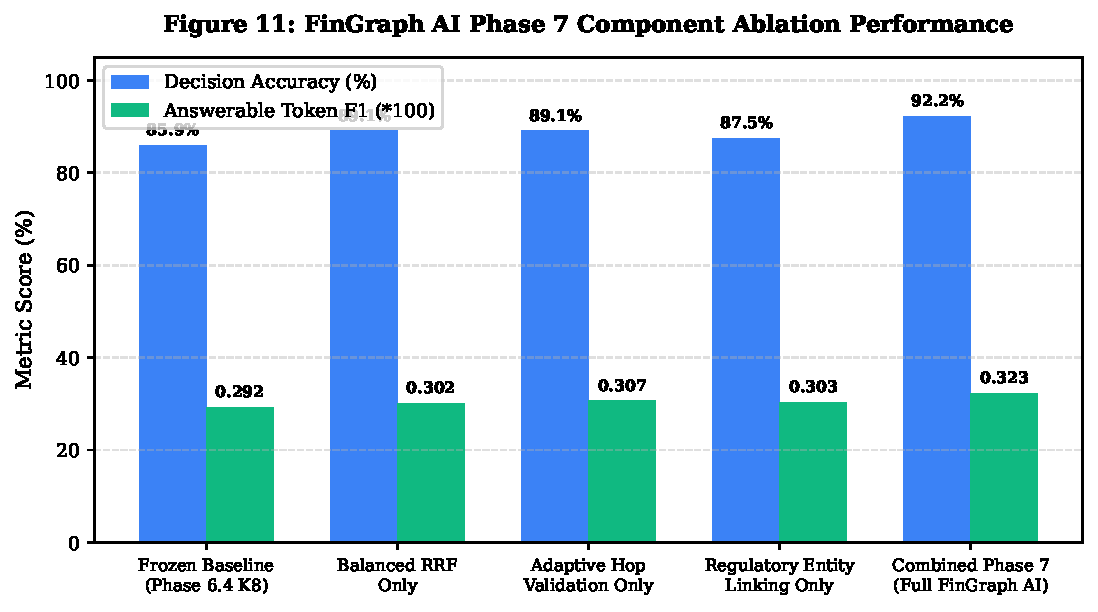
\includegraphics[width=\columnwidth]{../figures/fig11_ablation_results.pdf}
\caption{Component ablation across evaluation iterations.}
\label{fig:ablation}
\end{figure}

\section{Downstream Application: Return Forecasting}
To demonstrate the broader utility of our structured SEC ingestion pipeline, we evaluate an auxiliary 5-day stock return direction prediction task on 354 chronological snapshots of AAPL data (283 training, 71 testing). Combining market indicators with SEC filing velocity features (`MARKET + SEC V3`) yields a test ROC-AUC of 0.6342 and accuracy of 64.79\%, outperforming the Market-Only baseline (ROC-AUC 0.6096, accuracy 52.11\%), confirming the predictive information content embedded within regulatory disclosures.

\begin{figure}[t]
\centering
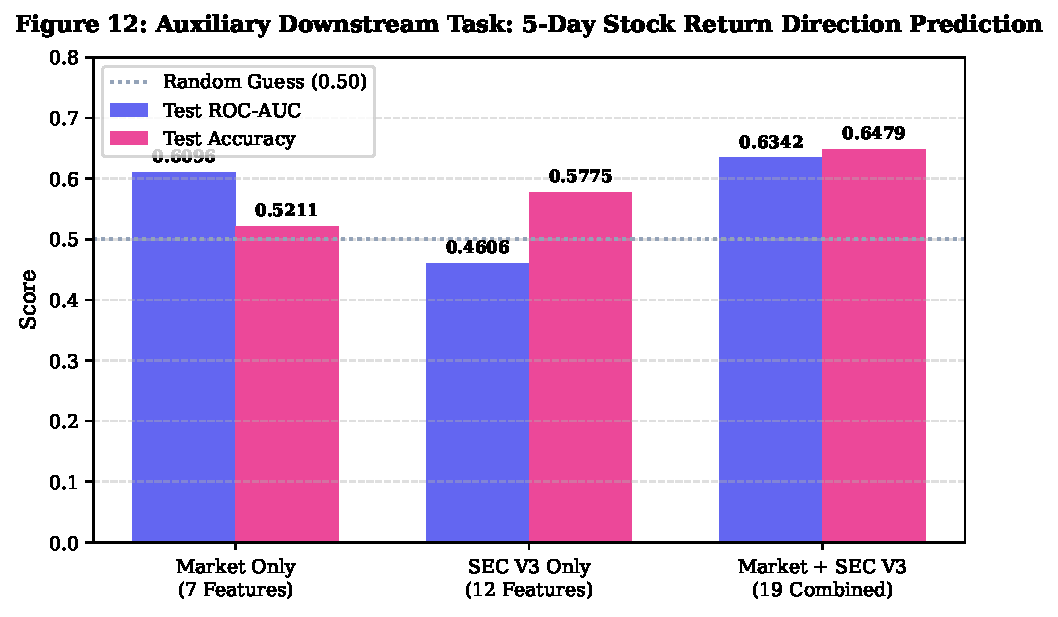
\includegraphics[width=0.85\columnwidth]{../figures/fig12_auxiliary_prediction.pdf}
\caption{Auxiliary 5-day stock return direction prediction performance.}
\label{fig:pred}
\end{figure}

\section{Threats to Validity \& Limitations}
\textbf{Benchmark Scale:} While densely curated and verified, the 64-question benchmark represents 10 large-cap US corporations. Expanding the corpus to mid-cap and cross-border filings is a key direction.  
\textbf{Generator Dependency:} The current deployment evaluates local `qwen3.5:4b`. While demonstrating edge efficiency, testing larger models (e.g. Llama 3.1 70B) may further improve descriptive Token F1.

\section{Conclusion}
We presented FinGraph AI, a temporal knowledge graph and hybrid GraphRAG framework for multi-hop financial question answering over SEC filings. Through Bitemporal Snapshot Slicing, Entity-Balanced RRF, and Adaptive Hop Gating, FinGraph AI achieves 92.19\% Decision Accuracy, zero temporal infiltration ($\text{FEIR}=0.0\%$), and 100\% refusal recall with zero hallucinations on unanswerable questions. All datasets, models, and interfaces are openly reproducible.

\bibliographystyle{IEEEtran}
\bibliography{references}

\end{document}
